\documentclass[reqno]{amsart}
\usepackage[margin=2.5cm]{geometry}
\usepackage{parskip}
\usepackage{graphicx}
\usepackage{float}
\usepackage{xcolor}
\linespread{1.5}

\usepackage{hyperref}
\usepackage{enumitem}
\renewcommand{\labelenumi}{$(\roman{enumi})$}
\renewcommand{\labelitemi}{$\cdot$}
\usepackage{mathtools}
\usepackage{amssymb}
\usepackage{amsmath}
\usepackage{mathrsfs}
\usepackage{booktabs}
\newcommand{\1}{\mathbbm{1}}
% measures / sets of measures:
\newcommand{\mH}{\mathscr{H}}
\newcommand{\mL}{\mathscr{L}}
\newcommand{\mP}{\mathscr{P}}
\newcommand{\cT}{\mathcal{T}} % topology
\newcommand{\cB}{\mathcal{B}} % borel
\newcommand{\W}{\mathcal{W}} % new metric W
\newcommand{\X}{\mathcal{X}} % space X
\newcommand{\Y}{\mathcal{Y}} % space Y
\newcommand{\expv}{\mathbb{E}} % exp value

\newcommand{\F}{\mathcal{F}} % space F
\newcommand{\M}{\mathcal{M}} % space of measures

\newcommand{\deriv}[2]{\frac{\de #1}{\de #2}}
\newcommand{\pderiv}[2]{\frac{\partial #1}{\partial #2}}
\newcommand{\sgn}[0]{\mathrm{sign}}

\newcommand{\nabladot}{\nabla \cdot} % discrete divergence operator
\newcommand{\A}{\mathcal{A}} % action
\newcommand*\de{\mathop{}\!\,\,\mathrm{d}}
\DeclareMathOperator*{\argmin}{arg\,min}
\DeclareMathOperator*{\argmax}{arg\,max}
\DeclareMathOperator*{\supp}{supp}
\DeclareMathOperator*{\id}{id}
\DeclareMathOperator{\imm}{Im}
\DeclareMathOperator{\lalpha}{\overline{\alpha}}
\DeclareMathOperator{\aconv}{\alpha \textit{x}+\overline{\alpha}\textit{y}}
\DeclareMathOperator{\bconv}{\beta \textit{x}+\overline{\beta}\textit{y}}

%%%%%%%%%%%%%%%%%%%% from the paper
\newcommand{\R}{\ensuremath{\mathbb{R}}}
\newcommand{\N}{\ensuremath{\mathbb{N}}}
\newcommand{\Z}{\ensuremath{\mathbb{Z}}}
\newcommand{\card}{\vert\mathscr{H}\vert} % |H|
\newcommand{\LL}{\mathscr{L}}
\newcommand{\PP}{\mathbb{P}}
\newcommand{\hyp}{\mathscr{H}}

\newcommand{\Rad}{\widehat{\mathfrak R}_D}


\DeclareMathOperator{\Ric}{Ric}
\DeclareMathOperator{\vol}{vol}
\DeclareMathOperator{\Var}{Var}

\def\diam{\mathop{\mathrm{diam}}\nolimits}
\def\vol{\mathop{\mathrm{vol}}\nolimits}
\def\area{\mathop{\mathrm{area}}\nolimits}
\def\Hess{\mathop{\mathrm{Hess}}\nolimits}
\def\supp{\mathop{\mathrm{supp}}\nolimits}
\def\Ric{\mathop{\mathrm{Ric}}\nolimits}
\def\Id{\mathop{\mathrm{Id}}\nolimits}
\def\tr{\mathop{\mathrm{tr}}\nolimits}
\def\ac{\mathop{\mathrm{ac}}\nolimits}
\def\div{\mathop{\mathrm{div}}\nolimits}
\def\proj{\mathop{\mathrm{proj}}\nolimits}

%%%%%%%%%%%%%%%%%%%%%%%%%%%%%%%%%%%%

\theoremstyle{plain}
\newtheorem{definition}{Definition}[section]
\newtheorem{proposition}[definition]{Proposition}
\newtheorem{theorem}[definition]{Theorem}

\newtheorem{corollary}[definition]{Corollary}
\newtheorem{lemma}[definition]{Lemma}
\newtheorem{example}[definition]{Example}
\newtheorem{remark}[definition]{Remark}
\newtheorem{assumption}[definition]{Assumption}
\newtheorem{fact}[definition]{Fact}

\newenvironment{intuition}[1][Intuition]{\begin{proof}[#1]\renewcommand{\qed}{\relax}}{\topsep0pt\end{proof}}

\newcommand{\mati}[1]{\textcolor{magenta}{#1}}

\title{Recap}
\author{Matilde Dolfato}

\raggedbottom
\begin{document}

\maketitle

{\bf Hyperparameters}

Labels are generated as
\[
y \leftarrow \sgn\left(5\, \sin\left(\frac{\pi \,( m  +1)}{10}\, x\right) + \sigma\varepsilon\right), \qquad \varepsilon\sim\mathcal N(0,1),
\]
with $x$ sampled uniformly from $N$ evenly spaced points of $(0,10)$. The noise level $\sigma$ is chosen so that the average flip probability $\frac{1}{N}\sum_{j}\Phi\left(-\vert h^*(\bar x_j)\vert/\sigma\right)$ equals the target percentage of flipped labels.

\begin{table}[h!]
\centering
\begin{tabular}{lll}
\toprule
Parameter & Symbol & Value \\
\midrule
Support size & $N$ & $10^9$ \\
Train size & $n$ & $500$ \\
Test size & $n_\text{test}$ & $200,000$ \\
Iterations & $T$ & $100$ \\
Crossings of $h^*$ & $m$ & $10$ \\
Noise & $\sigma$ & $\approx 3.5$, $20\%$ flipped labels \\
Depths & $d$ & $1,\ldots,\lfloor 4\log_2 n\rfloor$ \\
Constant, union bound & $C_\text{union}$ & $6\cdot 10^{-4}$ \\
Constant, Rademacher--Massart & $C_\text{radmass}$ & $0.125$ \\
Constant, noise bound & $C_\text{noise}$ & $0.01$ \\
Seed & & $4$ \\
\bottomrule
\end{tabular}
\end{table}

See Appendix~\ref{app: constants} for the computation of the constants.

\begin{figure}[H]
  \centering
  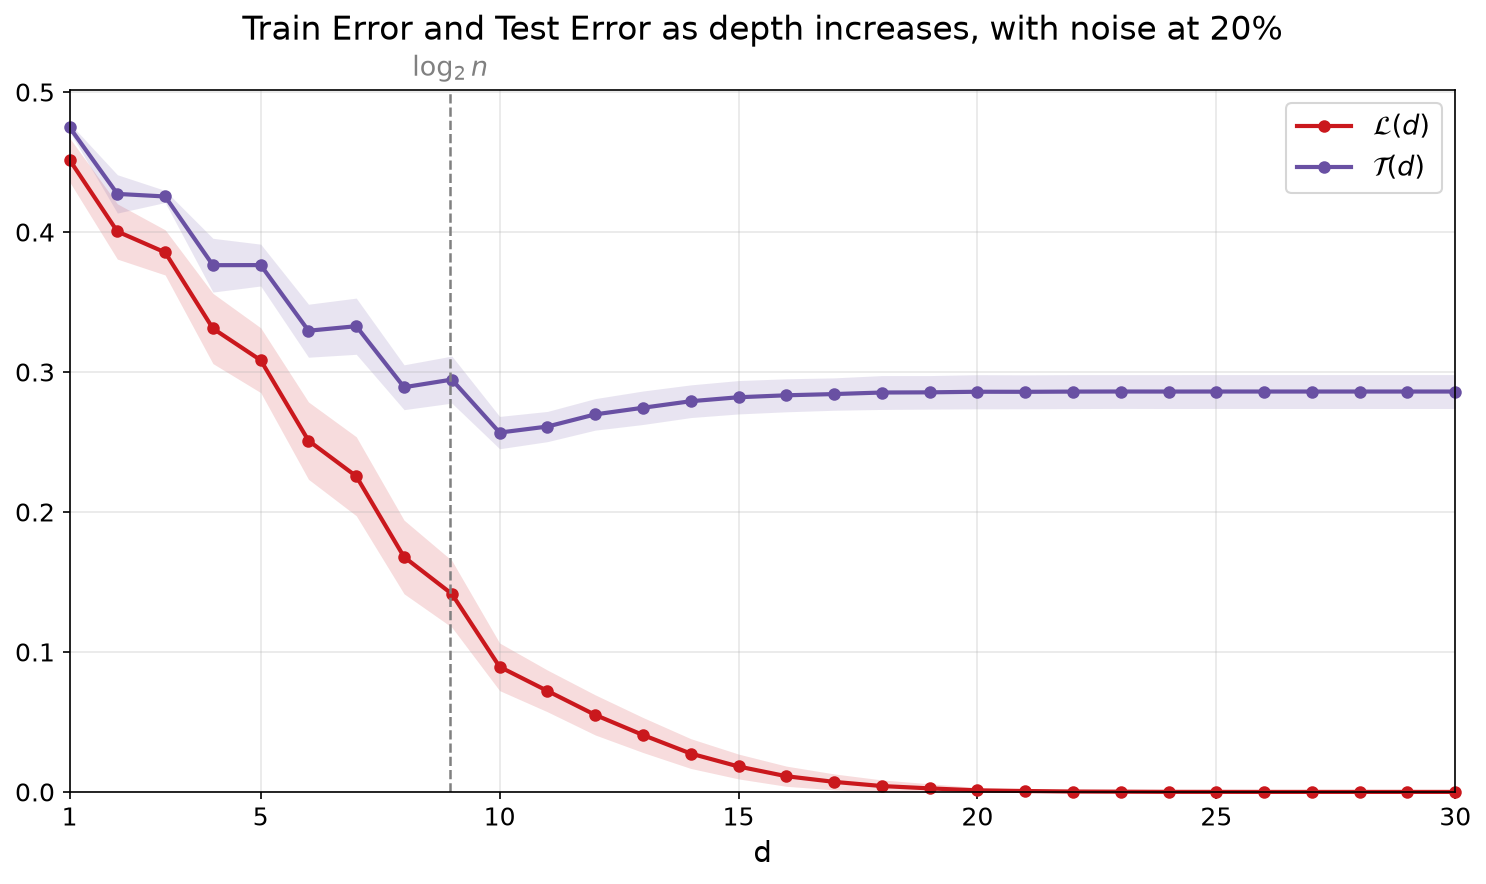
\includegraphics[width=\textwidth]{outputs/train_test.png}
  \caption{Train and test error as functions of the maximum depth $d$.}
  \label{fig:train test}
\end{figure}

{\bf Hypotheses class}

Consider the algorithm of binary decision trees with test at nodes $x\ge t$ for arbitrary $t\in\R$. 
When $\hyp_d$ is the class of functions represented by such trees of depth at most $d$,
\[
\vert\hyp_d\vert = 2 \sum_{j = 0}^{\min\{2^d -1, N-1\}}\binom{N-1}{j}
\]
which yields
\[
\log \vert\hyp_d\vert = (2^d -1) \log{\frac{eN}{2^d}} = O(2^d) \qquad \text{for } d \ll \log_2 N
\]
and
\[
\log \vert\hyp_d\vert = N\log 2 \qquad \text{for } d \ge \log_2 N.
\]

\newpage
\section{Union bound}

\begin{theorem}\label{thm: unionbound} Let $\ell$ be bounded, $\ell(\cdot) \le M$ for some $M\in\R$. Then
\[
  0 \le \expv[(R - \hat R_D)(\hat h_D)] \le 2M\sqrt{\frac{\log \vert \hyp \vert}{2n}}
\]
\end{theorem}

With the zero-one loss and $\hyp = \hyp_d$, we plot
\[
6\cdot 10^{-4}\cdot 2\sqrt{\frac{\log \vert \hyp_d \vert}{2n}}
\]

\begin{figure}[H]
  \centering
  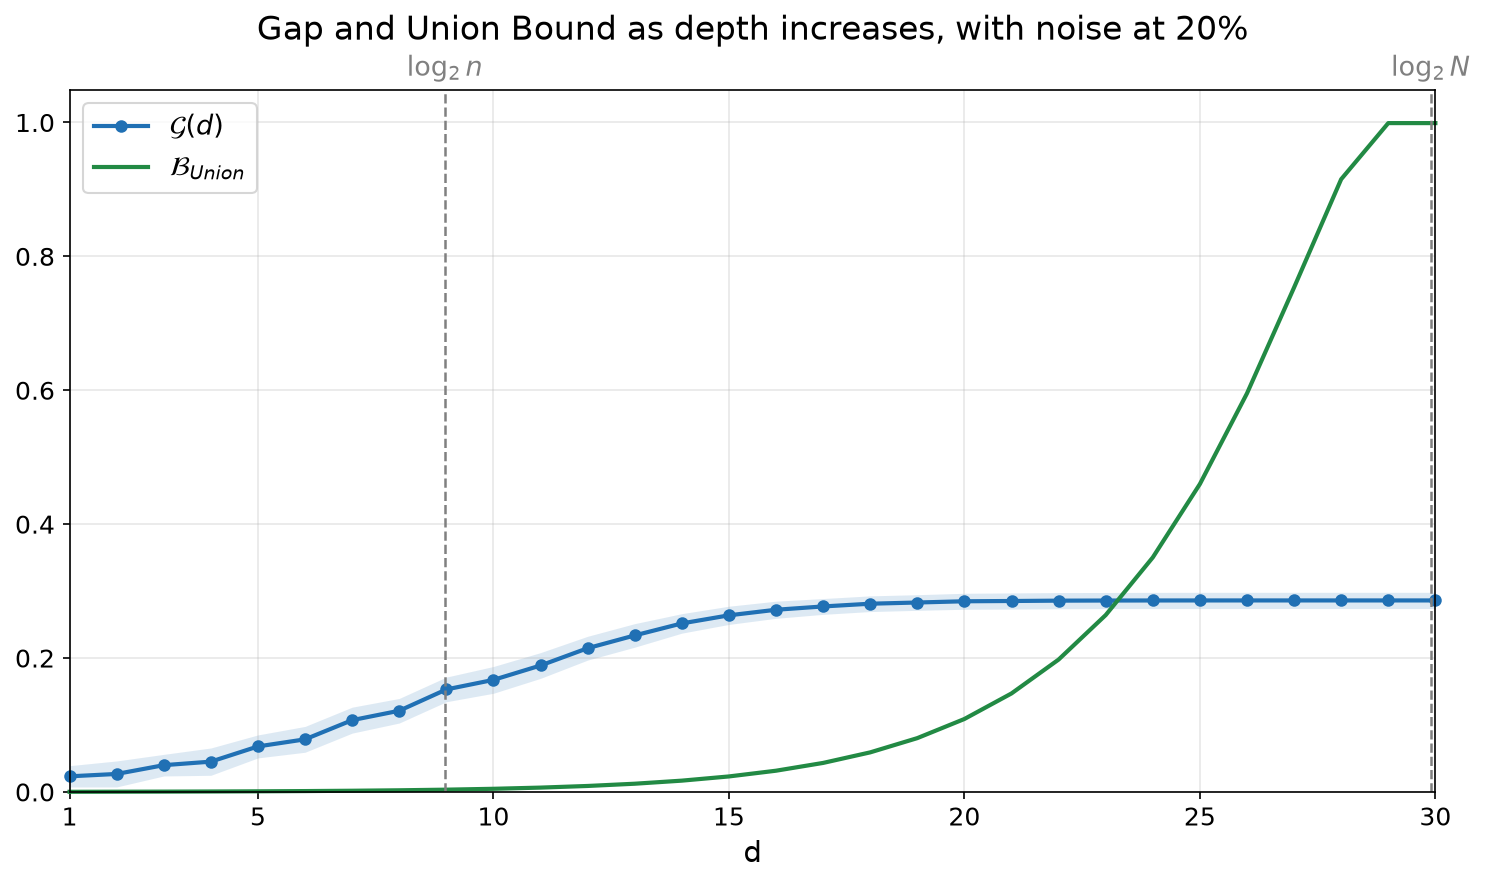
\includegraphics[width=\textwidth]{outputs/union_bound.png}
  \caption{Union bound (Theorem~\ref{thm: unionbound}) against the gap.}
  \label{fig:union bound}
\end{figure}

The generalization gap saturates around $d = 15$, slightly after the interpolation threshold $\lceil\log_2 n\rceil = 9$. The bound, instead, saturates at $\log_2 N = 30$. This bound does not capture well the shape of the generalization gap, in fact it is myopic to the algorithm. Indeed, if we didn't discretize the support, i.e.\ we let $N \to \infty$, the saturating value would be infinite. 

\begin{figure}[H]
  \centering
  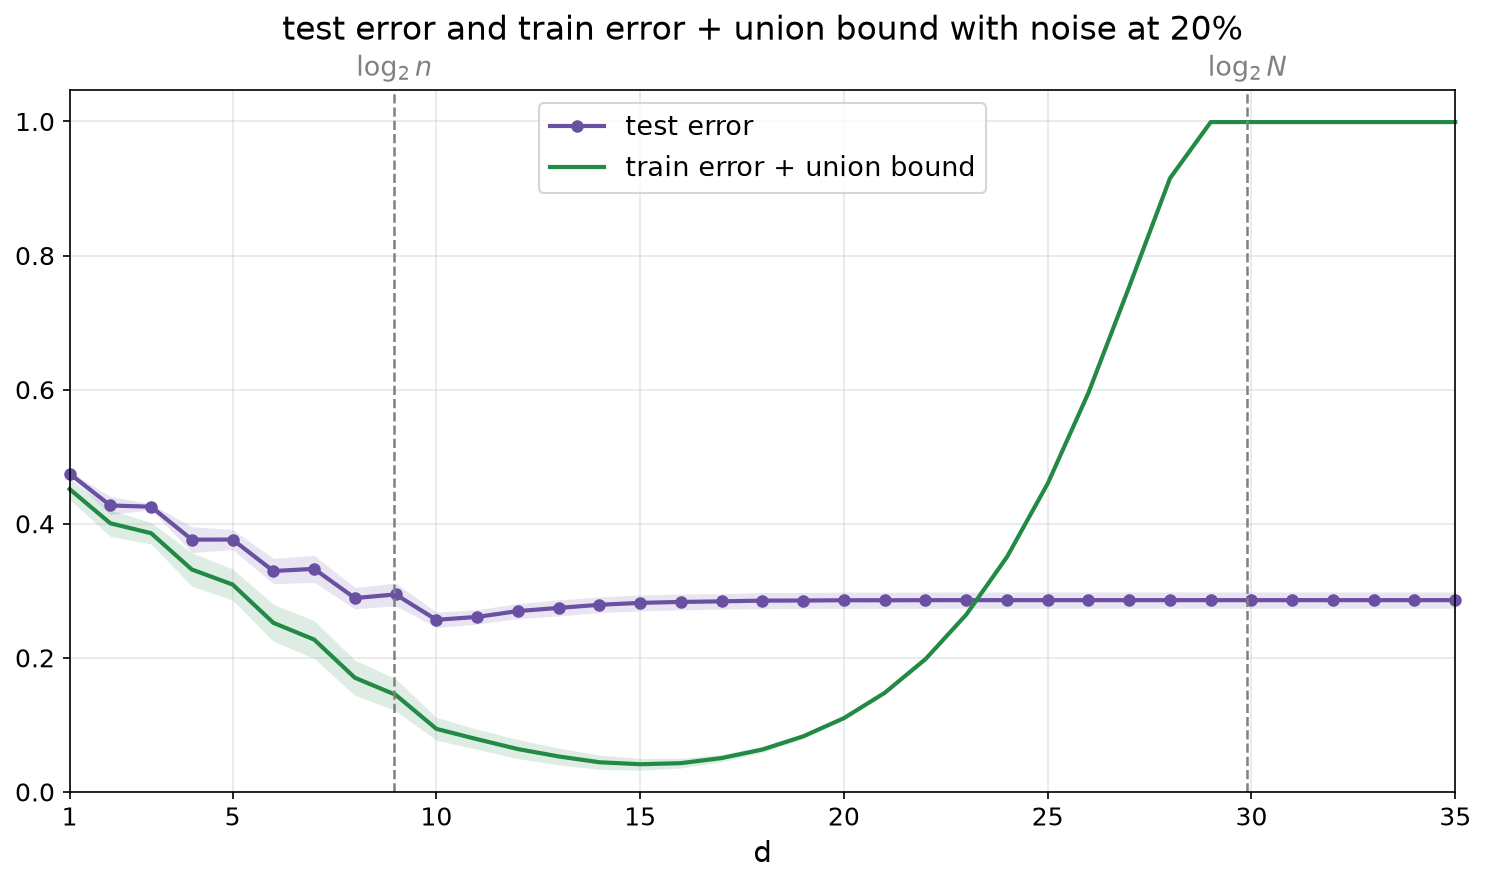
\includegraphics[width=\textwidth]{outputs/train_union_bound.png}
  \caption{Test error against union bound (Theorem~\ref{thm: unionbound}) plus train error.}
  \label{fig:union bound trainerr}
\end{figure}

\newpage
\section{Rademacher and Massart bound}

Let \[N_D(\hyp)\coloneq \left\vert\left\{\left(\ell_h(X_1,Y_1),\ldots,\ell_h(X_n,Y_n)\right) : h\in\hyp, D = {((X_i, Y_i))}_{i=1}^n\right\}\right\vert\] be the cardinality of the set of loss vectors for the hypotheses in $\hyp$, which is a random variable as it depends on the dataset $D$.

\begin{theorem}[Rademacher and Massart bound]\label{thm: rademmassart ND} Let $\ell$ be the zero-one loss. Then
\[
\expv[(R-\hat R_D) (\hat h_D)]\le 2\sqrt{\frac{2\log \expv[N_D(\hyp)]}{n}}
\]
\end{theorem}

\begin{lemma}[Counting]\label{lemma: counting} Let $\ell$ be the zero-one loss. Then
\[
N_{D}(\hyp) \le \min\{\vert\hyp\vert, 2^n\}
\]
surely.
\end{lemma}

Substituting Lemma~\ref{lemma: counting} into Theorem~\ref{thm: rademmassart ND}, we obtain the following.

\begin{corollary}\label{thm: rademmassart bound} Let $\ell$ be the zero-one loss. Then
\[
\expv[(R-\hat R_D) (\hat h_D)]\le \min\left\{2\sqrt{\frac{2\log\card}{n}}, 2\sqrt{2\log 2}\right\}
\]
\end{corollary}

With the zero-one loss and $\hyp = \hyp_d$, we plot
\[
0.125\cdot\min\left\{2\sqrt{\frac{2\log\vert\hyp_d\vert}{n}}, 2\sqrt{2\log 2}\right\}
\]

\begin{figure}[H]
  \centering
  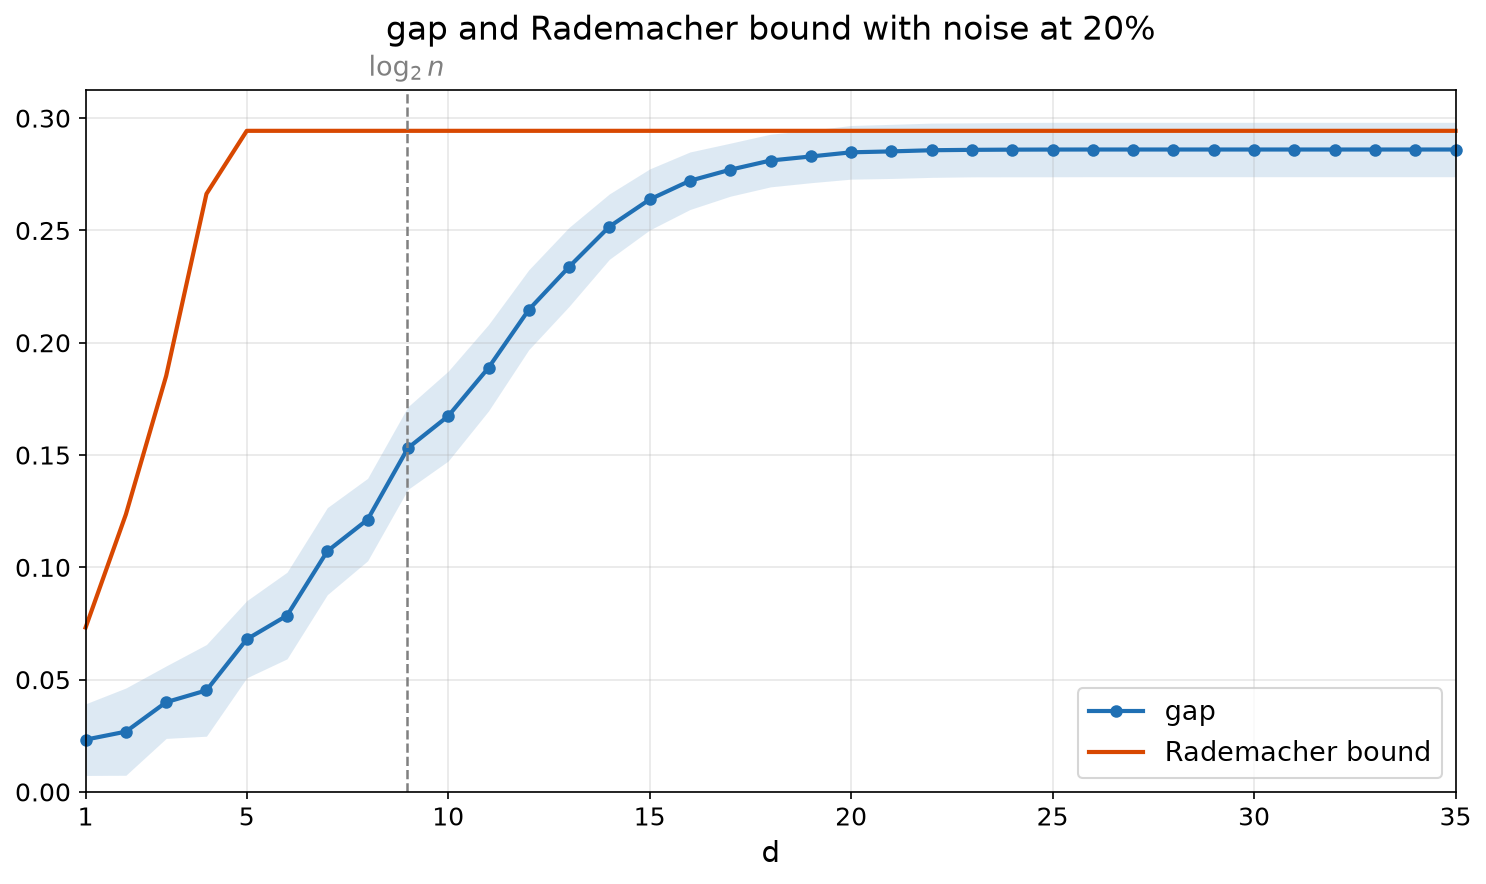
\includegraphics[width=\textwidth]{outputs/radmass_bound.png}
  \caption{Rademacher and Massart bound (Corollary~\ref{thm: rademmassart bound}) against the gap.}
  \label{fig:radmass bound}
\end{figure}

The bound obtained in Corollary~\ref{thm: rademmassart bound} better captures the curve of the test error, because it saturates from a lower depth. Specifically, for low values of the depth $d$, the minmum in Lemma~\ref{lemma: counting} is attained by $\vert \hyp_d\vert$, while for a large enough depth the minimum becomes $2^n$ and the curve saturates. The depth at which the bound saturates is given by
\[
\log \vert \hyp_d\vert = (2^d-1)\log{\frac{eN}{2^d}} \ge n \quad \Rightarrow \quad d \ge 5
\]
for a fixed $n = 500$. 

\begin{figure}[H]
  \centering
  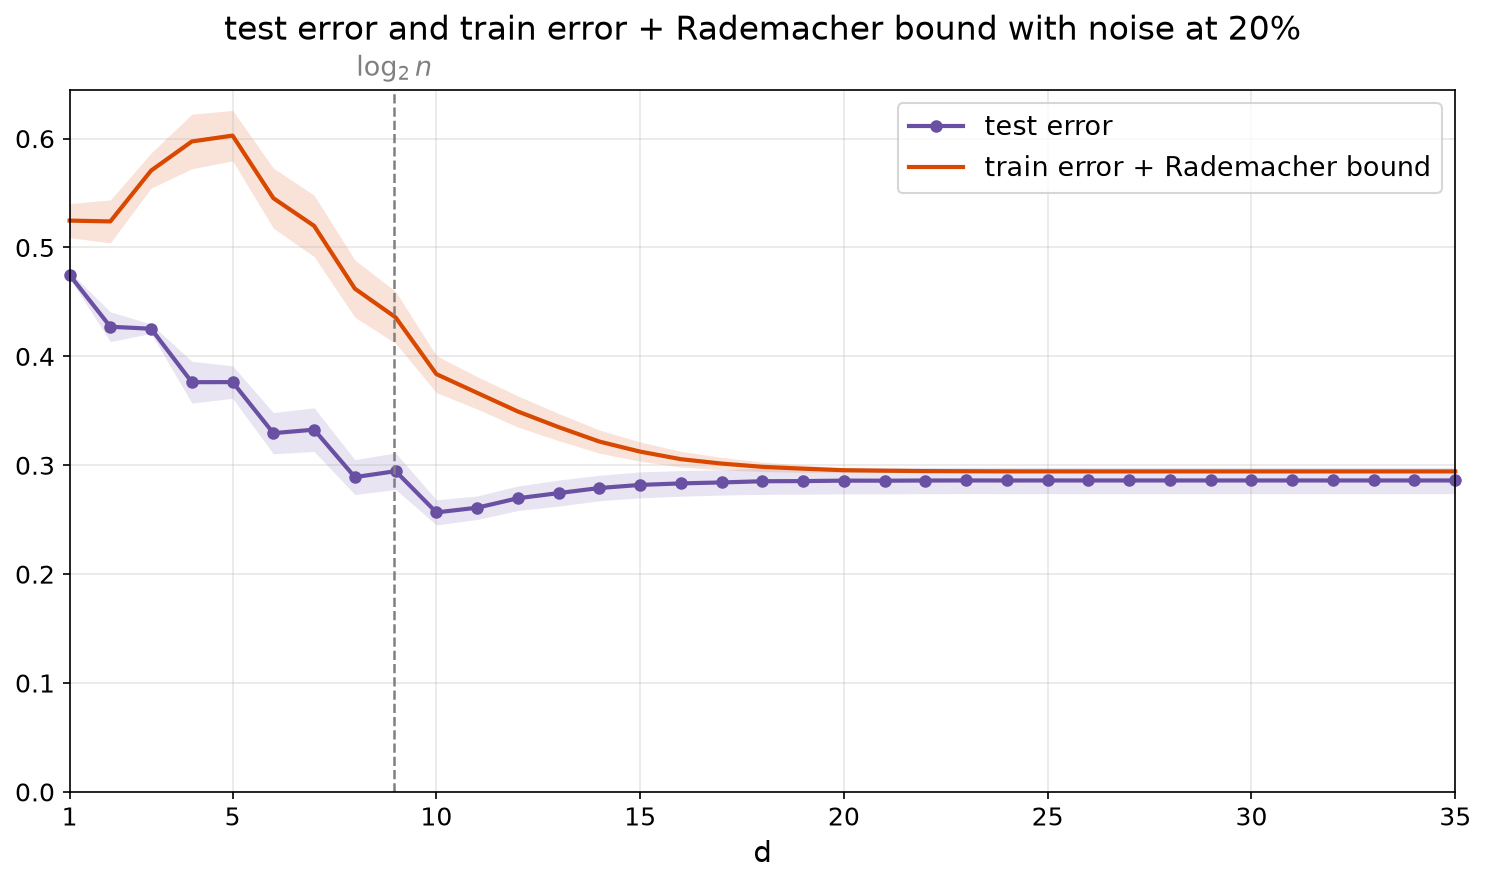
\includegraphics[width=\textwidth]{outputs/train_radmass_bound.png}
  \caption{Test error against Rademacher and Massart bound (Corollary~\ref{thm: rademmassart bound}) plus train error.}
  \label{fig:radmass bound trainerr}
\end{figure}

{\bf Comparison with the union bound}

Up to constants, the first term in the minimum of Corollary~\ref{thm: rademmassart bound} is the union bound of Theorem~\ref{thm: unionbound}. The two bounds coincide as long as $\log\vert\hyp_d\vert < n\log 2$, i.e.\ $\vert\hyp_d\vert < 2^n$, which with $n = 500$ and $N = 10^9$ holds for $d\le 4$. From $d = 5$ onwards, the minimum is attained by the constant term and the Rademacher and Massart bound saturates, while the union bound keeps increasing up to $d = \log_2 N$.

\begin{figure}[H]
  \centering
  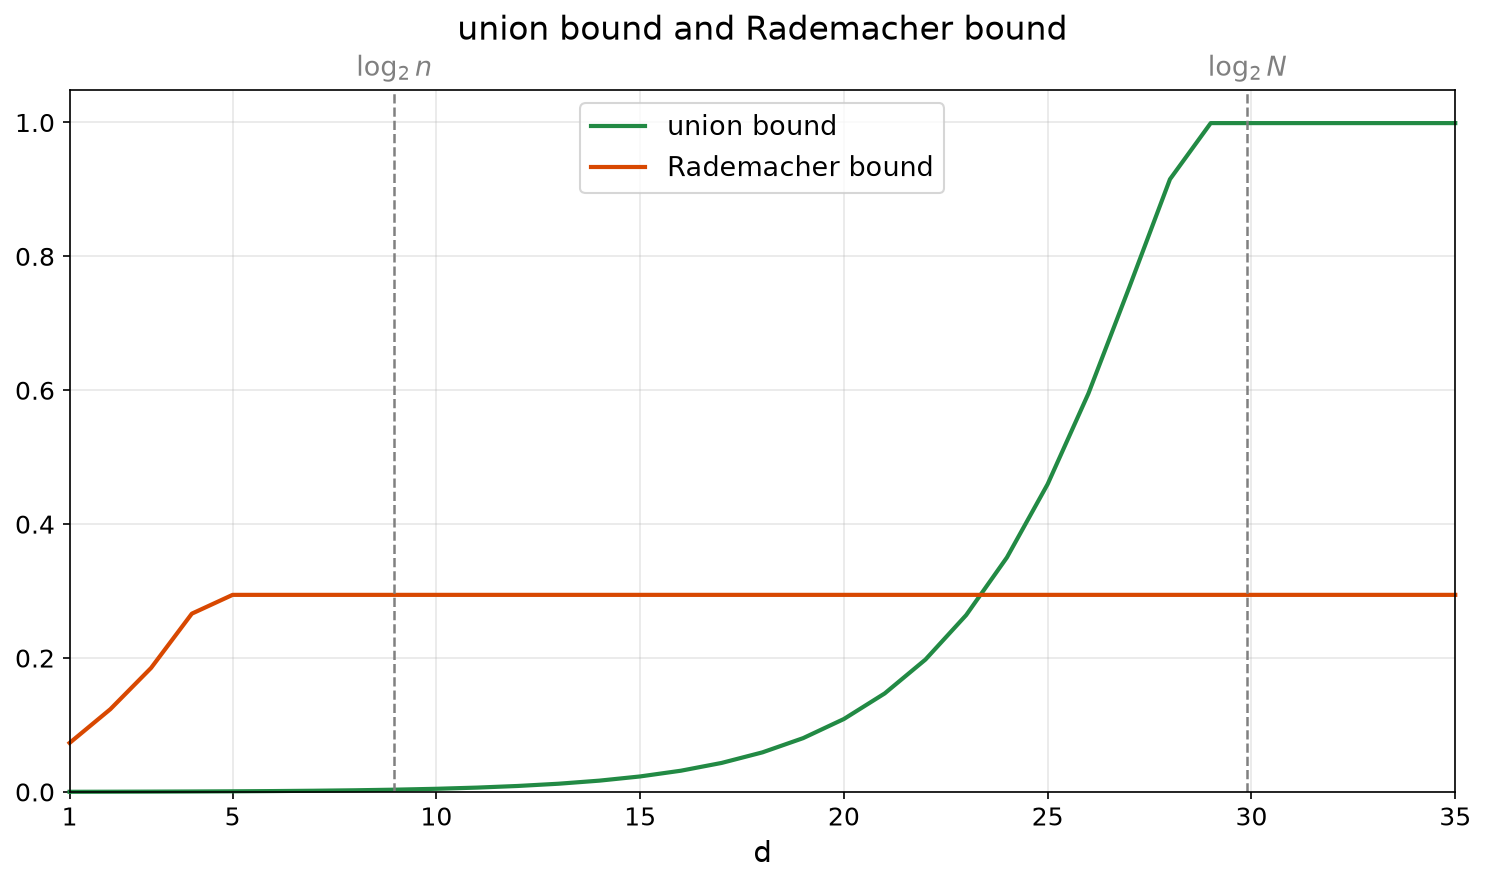
\includegraphics[width=\textwidth]{outputs/union_bound_radmass_bound.png}
  \caption{Union bound (Theorem~\ref{thm: unionbound}) against Rademacher and Massart bound (Corollary~\ref{thm: rademmassart bound}).}
  \label{fig:union radmass}
\end{figure}

{\bf Dependence on the noise}

The bound of Corollary~\ref{thm: rademmassart bound} does not depend on the noise, while the gap does: with $5\%$, $20\%$ and $40\%$ of flipped labels, it saturates at different levels, as shown in Figure~\ref{fig:radmass noise}.

\begin{figure}[H]
  \centering
  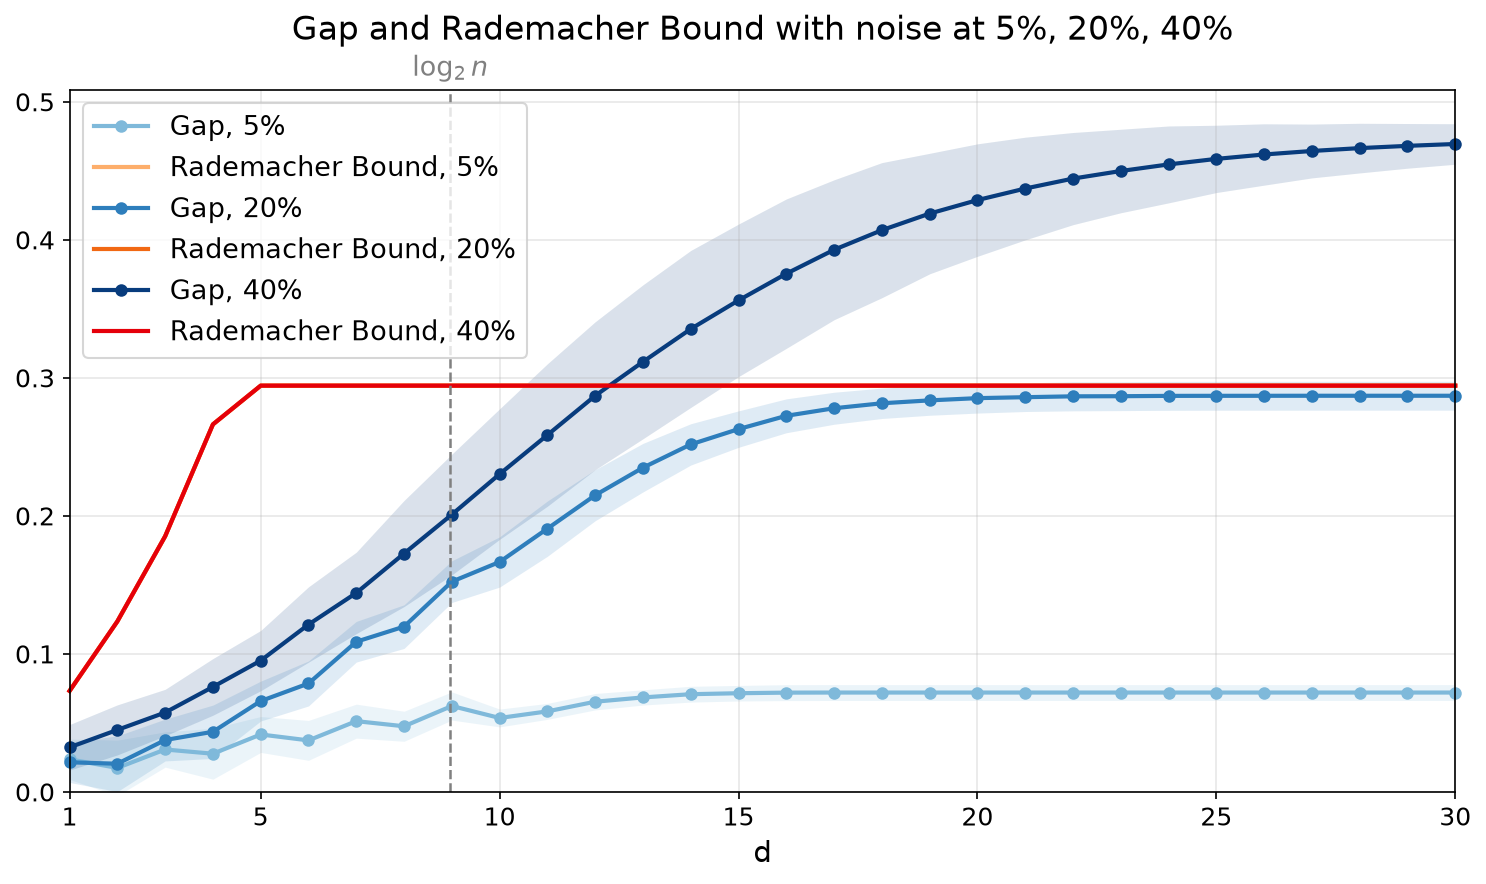
\includegraphics[width=\textwidth]{outputs/radmass_bound_many_noise.png}
  \caption{Rademacher and Massart bound (Corollary~\ref{thm: rademmassart bound}) against the gap for different noise levels.}
  \label{fig:radmass noise}
\end{figure}

\newpage
\section{Noise and approximation error bound}

Let $R^*_\hyp = \min_{h\in\hyp} R(h)$ be the best risk, $R^* = \inf_{h:\X\to\Y} R(h)$ the Bayes risk and $A_\hyp = R^*_\hyp - R^*$ the approximation error.

\begin{theorem}[Noise and approximation error bound]\label{thm: bound noiseandappr}
  Let $\ell$ be the zero-one loss. Then
  \begin{equation*}
\begin{split}
\expv\left[(R-\hat R_D)(\hat h_D)\right] \le \min\Bigg\{ &4\sqrt{\frac{(R^*+A_{\hyp})\left(\log (4\card)+1\right)}{n}} + 20\,\frac{\log(4\card)+1}{n}, \\
&4\sqrt{\frac{(R^*+A_{\hyp})\left((2n+2)\log 2+1\right)}{n}} + 20\,\frac{(2n+2)\log 2+1}{n} \Bigg\}
\end{split}
\end{equation*}
\end{theorem}

With $\hyp = \hyp_d$, we plot
\[
0.01\cdot\min\left\{4\sqrt{R^*_{\hyp_d}L_d} + 20L_d,\ 4\sqrt{R^*_{\hyp_d}M} + 20M\right\}, \qquad L_d = \frac{\log (4\vert\hyp_d\vert)+1}{n},\quad M = \frac{(2n+2)\log 2+1}{n},
\]
where $R^*_{\hyp_d} = R^* + A_{\hyp_d}$ is computed exactly for each $d$ by dynamic programming.

\begin{figure}[H]
  \centering
  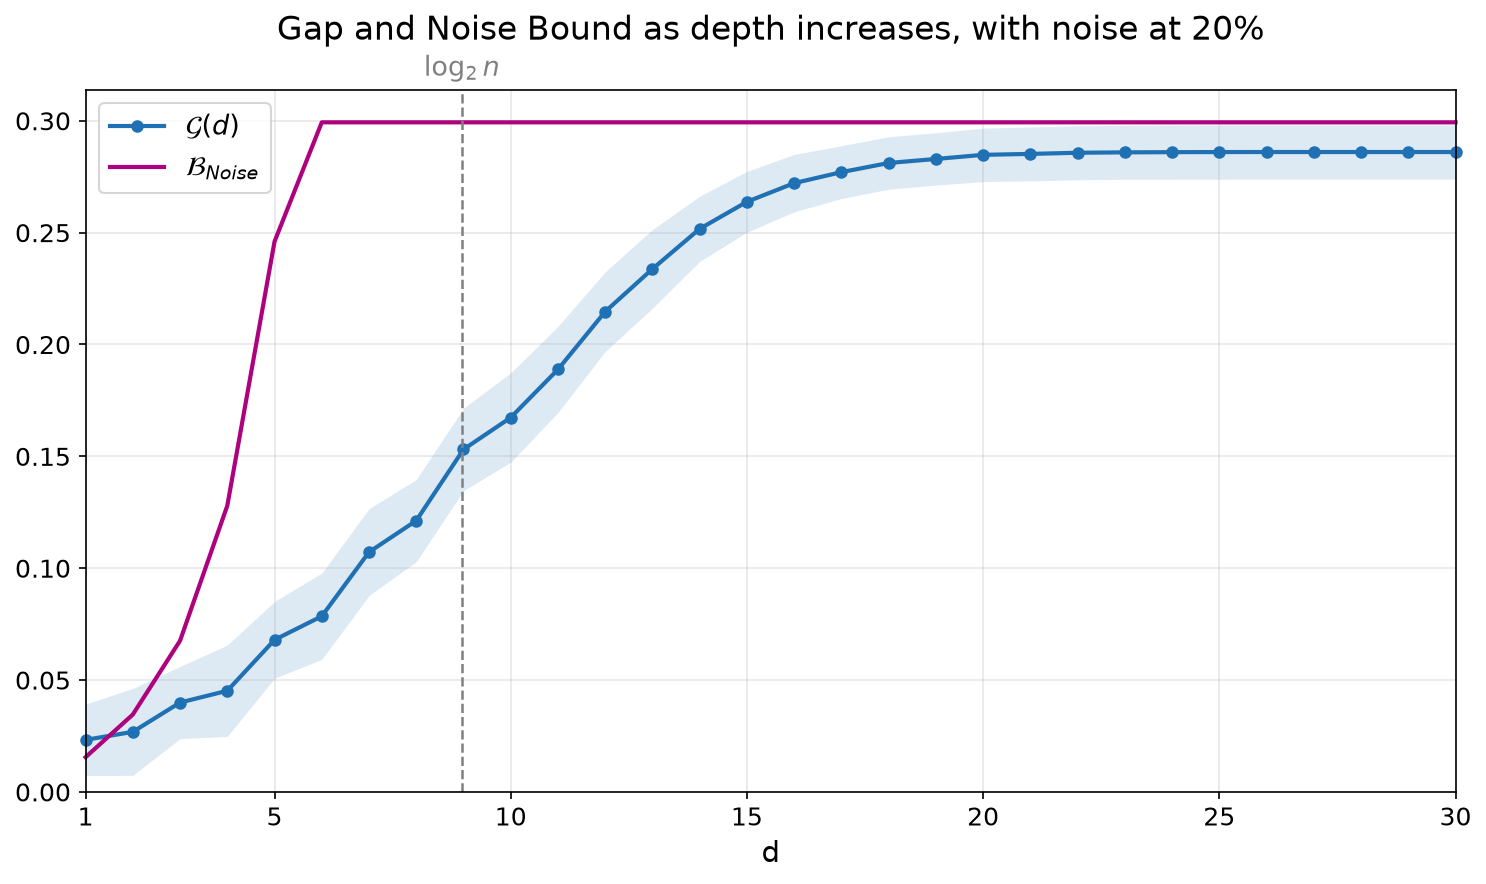
\includegraphics[width=\textwidth]{outputs/noise_bound.png}
  \caption{Noise and approximation error bound (Theorem~\ref{thm: bound noiseandappr}) against the gap.}
  \label{fig:noise bound}
\end{figure}

\begin{figure}[H]
  \centering
  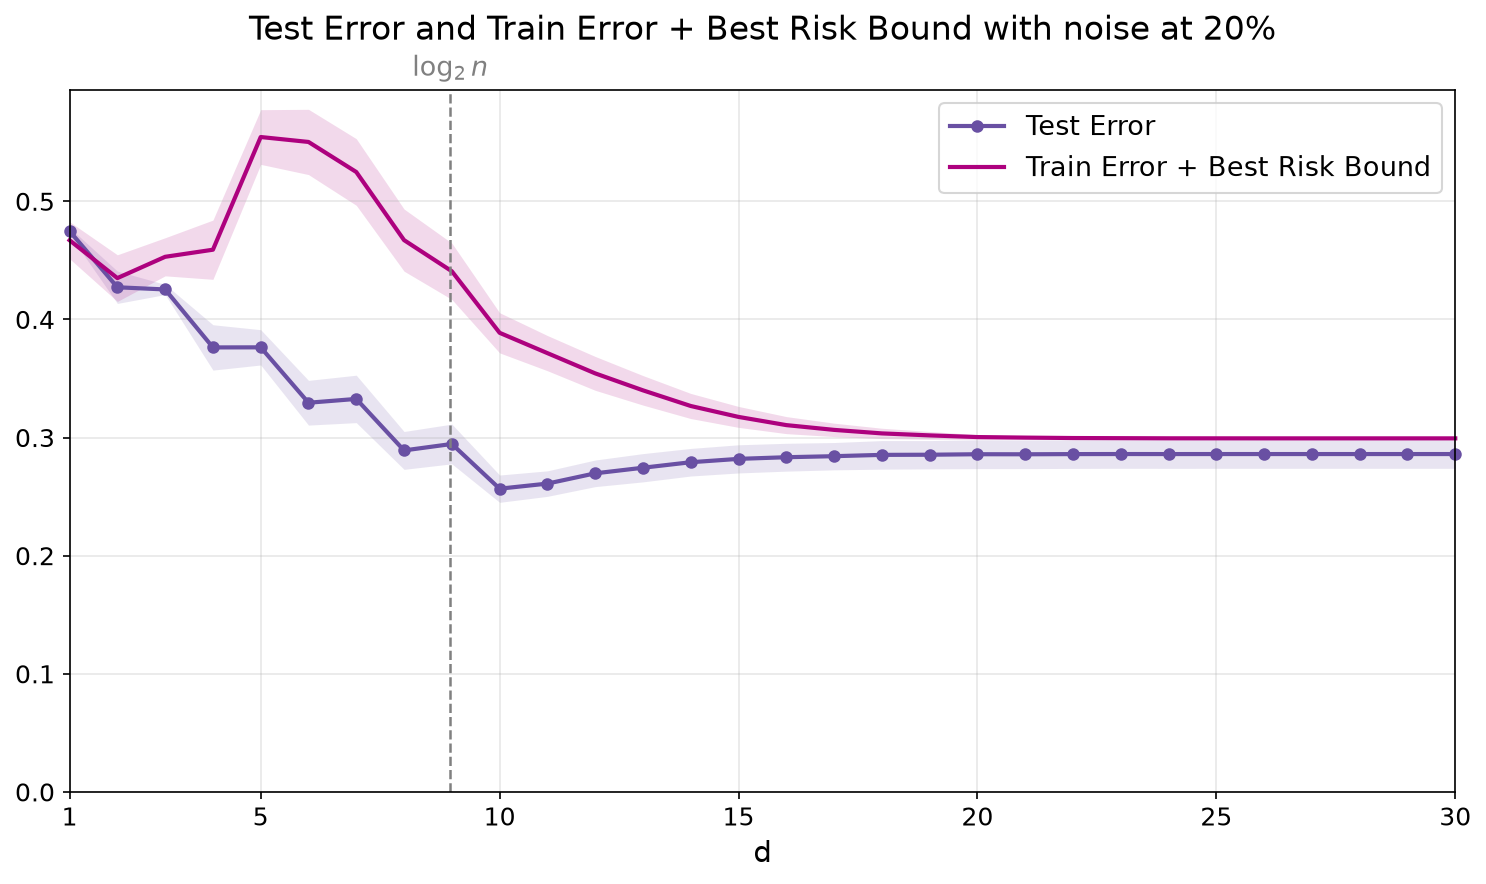
\includegraphics[width=\textwidth]{outputs/train_noise_bound.png}
  \caption{Test error against noise and approximation error bound (Theorem~\ref{thm: bound noiseandappr}) plus train error.}
  \label{fig:noise bound trainerr}
\end{figure}


{\bf Dependence on the noise}

\begin{figure}[H]
  \centering
  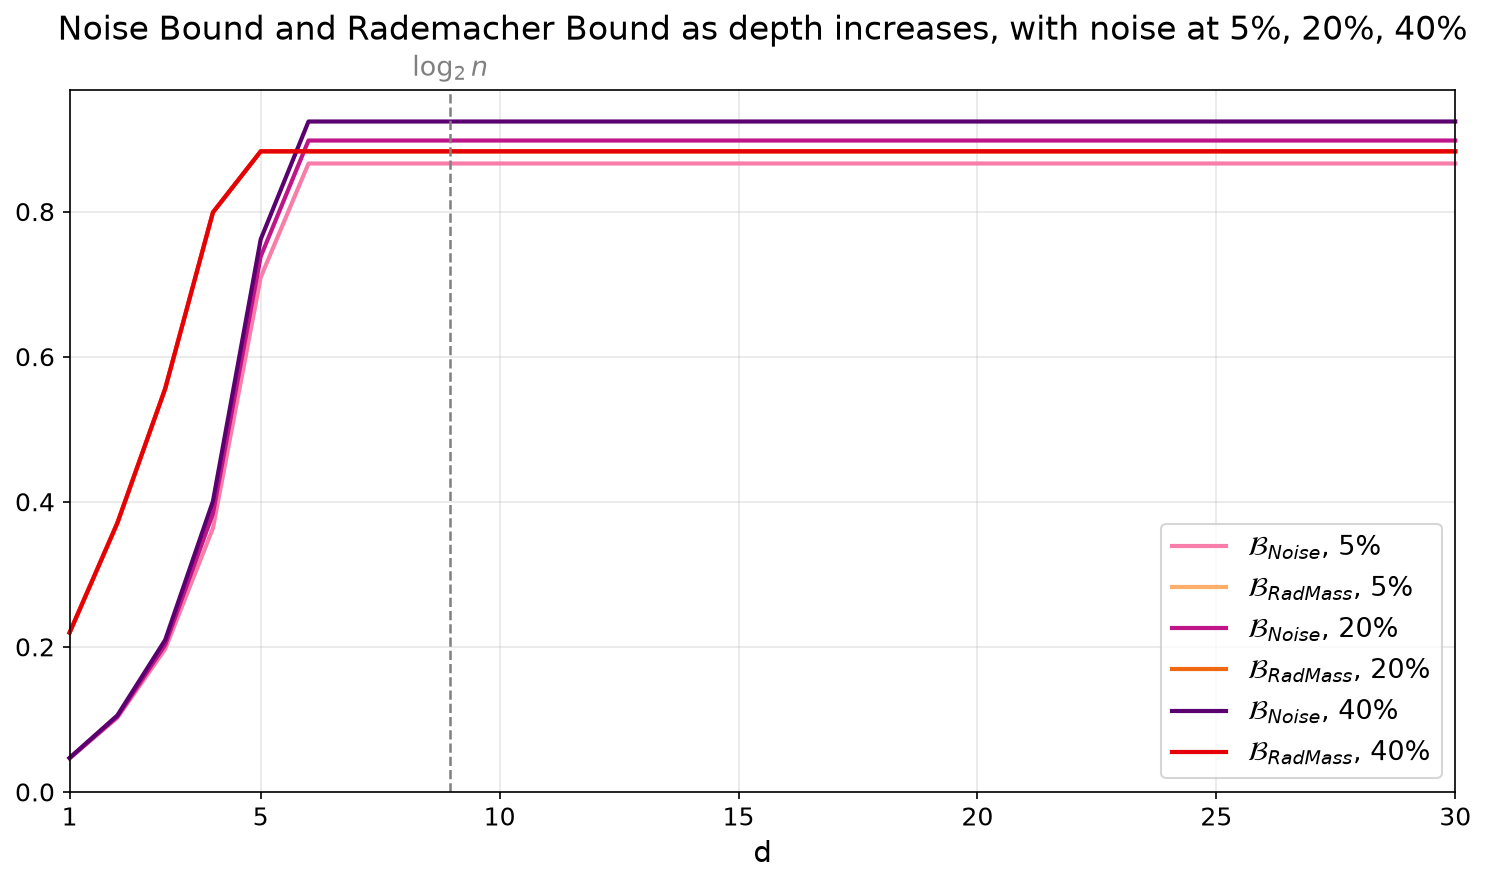
\includegraphics[width=\textwidth]{outputs/noise_bound_radmass_bound_many_noise.png}
  \caption{Noise and approximation error bound (Theorem~\ref{thm: bound noiseandappr}) against Rademacher and Massart bound (Corollary~\ref{thm: rademmassart bound}) for different noise levels.}
  \label{fig:noise radmass noise}
\end{figure}

Figure~\ref{fig:noise radmass noise} shows that the Rademacher and Massart bound does not change with the noise, while the noise and approximation error bound shifts upwards as the noise increases. Note that the constants used here are three times those used above ($0.375$ and $0.03$), to better visualize the differences in the noise and approximation error bound.

\begin{figure}[H]
  \centering
  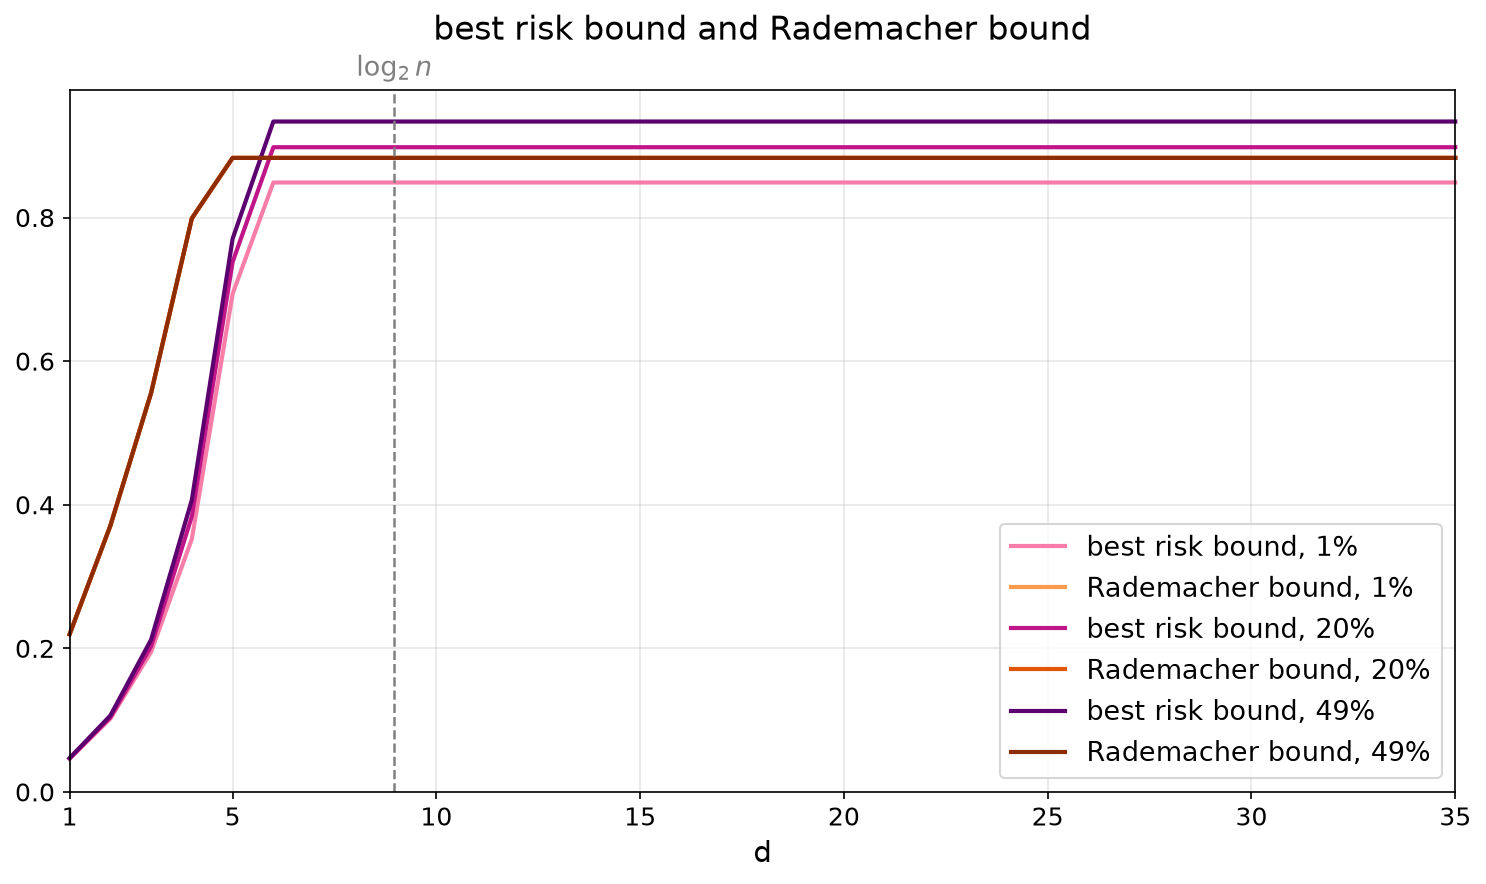
\includegraphics[width=\textwidth]{outputs/noise_bound_radmass_bound_many_noise_2.png}
  \caption{Noise and approximation error bound (Theorem~\ref{thm: bound noiseandappr}) against Rademacher and Massart bound (Corollary~\ref{thm: rademmassart bound}) for different noise levels (more extreme).}
  \label{fig:noise radmass extreme noise}
\end{figure}

Figure~\ref{fig:noise radmass extreme noise} is an attempt to vsiualize better the sensitivity of the noise bound using more extreme noise levels ($1\%$, $20\%$, $49\%$), with the same constants as in Figure~\ref{fig:noise radmass noise}, with poor results. 

\newpage
\appendix
\section{Fitting constants}\label{app: constants}

\paragraph{Union bound} We just rescale the bound so that it lies in the interval $[0,1]$. For $d$ large, $\log\vert\hyp_d\vert = N\log 2$. This means that the bound is $2 \sqrt{\frac{N\log 2}{2n}}$, hence we need
\[
C_\text{union}\cdot 2 \sqrt{\frac{N\log 2}{2n}} = 1
\]
Therefore we set
\[ C_\text{union} = \frac{1}{2 \sqrt{\frac{10^9\log 2}{2\cdot 500}}} = \frac{1}{2 \sqrt{ 10^6\log 2 }} = \frac{1}{2\sqrt{\log 2}}10^{-3} \approx 0.0006
\]


\paragraph{Rademacher and Massart bound} Using the code \texttt{source/experiments.py}, we print the value of the generalization gap for the highest depth $d=35$, getting 
\[
0.2860 \pm 0.0121
\]
Therefore, to obtain that the curve of the Rademacher bound saturates at the same level, we need
\[
C_{\text{RadMass}}2\sqrt{2\log 2} = 0.286 \quad \Rightarrow \quad C_{\text{RadMass}} = \frac{0.286}{2\sqrt{2\log 2}} = 0.12145302 \approx 0.125
\]
which we approximate in eccesso for the bound to lie above the curve. 


\paragraph{Noise bound} Similarly, we want the bound to saturate at the same level of the empirical gap curve. The saturating level of the bound, i.e.\ its value for a larghe depth, is 
\[
4\sqrt{R^*_{\hyp_d}M} + 20M \qquad \text{with }M = \frac{(2n+2)\log 2+1}{n}
\]
hence we set
\[
C_{\text{noise}} (4\sqrt{R^*_{\hyp_d}M} + 20M) = 0.286.
\]
We have 
\[
M = \frac{(1002)\log 2+1}{500} \approx 1.3910
\]
hence 
\[
(4\sqrt{R^*_{\hyp_d}M} + 20M) \approx 4 \sqrt{0.2\cdot 1.391} + 20\cdot 1.391 \approx 29.9298
\]
Thus,
\[
C_{\text{noise}} = 0.286 / 29.9298 \approx 0.01
\]
where we use $R^*_d = 0.2$ the Bayes risk, that is the value attained by the best risk for a large enough depth. 
\end{document}
